\chapter{Object-Caching}
\label{sec:object-caching}

Um die Dauer von Lesezugriffen im RMI-System zu verkürzen, wurde eine erweiterte Version des RMI-Systems mit integriertem Objectcaching erstellt. Schreibzugriffe werden an den Server gesendet. 

Bei der Erstellung des Konzeptes mussten Designentscheide in den Bereichen Replica Placement, Update Distribution und Konsistenzprotokoll getroffen werden. Im ersten Teil dieses Kapitels werden diese Entscheidungen beschrieben. Der zweite Teil beschreibt, wie diese Entscheide implementiert wurde.

Mit der Replikation von Objekten treten neue Probleme im Zusammenhang mit der Concurrency Control auf. Im Abschnitt \ref{sec:impl-der-conc} werden verschieden Ablaufszenarien untersucht, die zu Lost Updates führen.

\section{Replica Placement}
\label{sec:replica-management}

Ziel des Object Caching ist es, die Zugriffszeit auf Objekte für Clients zu verringern. Deshalb macht es Sinn, dass Repliken vom Client initiiert werden. Die Alternative wäre dass der Server die Repliken initiiert. Das macht Sinn, wenn der Server von Anfragen, die von den Repliken beantwortet werden können, entlastet werden soll. Werden die Replikas vom Client initiiert, spricht man von Client Caches. Client Caches verbessern die Zugriffszeit der Clients auf die Daten.

In unserem RMIwithObjectCaching-System besitzt jeder Client einen lokalen Cache auf seiner Maschine. Der Cache ist in der Grösse nicht limitiert, da es keine Testcases mit Szenarien, die mehrere Account-Objekte beinhalten, gibt. 

Durch das Caching sollen Lesezugriffe schneller ausgeführt werden, da der Aufruf nicht über ein Socket geschickt werden muss, sondern im RAM bleibt. Dies ist natürlich nur der Fall, wenn das Objekt im Cache vorhanden ist.

\section{Update Distribution}
\label{sec:update-distribution}

Werden Kopien von Objekten in einem lokalen Cache angelegt, müssen diese Kopien aktualisiert werden. Um dies zu realisieren gibt es mehrere Möglich\-keiten.

\subsection{Invalidation versus Data Transfer}
\label{sec:inval-vers-data}

\begin{description}
\item[Invalidation-Protocol] Bei einem Invalidation protocol werden nur Meldungen an die lokalen Caches gesendet, die dem Cache mitteilen, dass ein Objekt nicht mehr aktuell ist. Der Vorteil dieser Möglichkeit ist, dass eine Invalidierungsmeldung nur beim ersten Write versendet werden muss. Ausserdem müssen keine Objektdaten übertragen werden. Das Verfahren spart also Bandbreite. Ein Invalidation-Protocol macht Sinn, wenn das "'read-to-write-Verhältnis" klein ist.
\item[Transfer Data] Der zweite Ansatz ist, bei jedem Update die kompletten Daten eines Objektes an die lokalen Caches zu versenden. In diesem Fall kann der Client immer aus dem lokalen Cache lesen. Dieser Ansatz eignet sich bei einem hohen "'read-to-write Verhältnis".
\end{description}

Unser System verwendet den Transfer Data Ansatz, da in unseren Testszenarien sehr viele Lesezugriffe vorhanden sind. Das heisst, dass die Informationen in einem Update mit grosser Wahrscheinlichkeit im Cache gelesen werden. In diesem Fall müssen weniger Nachrichten versendet werden, wenn die aktualisierten Objekte bereits im lokalen Cache liegen. Bei einem Invalidation-Protocol müsste man jedes Mal eine aktualisierte Version anfordern.

\subsection{Pull versus Push}
\label{sec:pull-versus-push}

Die Verantwortung der Cache-Aktualisierung kann entweder beim Server oder beim Client liegen. Man unterscheidet zwischen "'push-based" und "'pull-based" Protokollen.

\begin{description}
\item[push-based] Der Server sendet dem Client Updates ohne, dass der Client diese anfordert. Der Server muss Buch darüber führen, in welchen Caches Kopien aller Objekte vorhanden sind.
\item[pull-based] Clients überprüfen bei jedem Zugriff, ob die Daten im Cache aktuell sind. Wenn nicht, müssen die Daten neu angefordert werden. Das macht den Zugriff auf Daten langsamer. Der Vorteil dabei ist, dass sich der Server nicht darum kümmern muss.
\end{description}

In unsererem Cache werden Aktualisierungen durch "'push-based" Updateds realisiert, da wir die Zugriffzeit für die Clients erhöhen wollen und sich die Anzahl der Clients in Grenzen hält. Der Server kann sich merken, welcher Cache welche Objekte enthält.

\section{Konsistenzprotokoll}
\label{sec:konsistenzprotokoll}

\subsection{Konsistenzmodell}
\label{sec:konsistenzmodell}

In unserem System greifen Client auf gemeinsame Objekte zu, indem sie Schreib- und Leseoperationen darauf ausführen. Jeder Client kann eine lokale Kopie eines Objektes bei sich im Cache haben. Führt eine Client eine Schreiboperation auf einem Objekt aus, muss diese durch das ganze verteilte System propagiert werden.
Ein Konsistenzmodel beschreibt unter anderem in welcher Reihenfolge die Clients die Schreiboperationen sehen. Das Konsistenzprotokoll implementiert das Konsistenzmodel.

Sequenzielle Konsistenz ist ein Konsistenzmodel. Es definiert, dass alle Prozesse in einem verteilten System die selbe Reihenfolge der Operationen auf einem Objekt sehen \cite{tanenbaum07}.  Das Konsistenzprotokoll unseres Object-Caching-Systems implementiert sequenzielle Konsistenz.

\subsection{Primary-Based Protokol}
\label{sec:prim-bnased-prot}

In unserem System sind alle Objekte zentral auf einem Server abgespeichert. Das Objekt auf dem Server ist das Referenzobjekt. Alle Schreiboperationen werden von den Clients an den Server gesendet. Die Reihenfolge der Schreiboperationen auf einem Objekt ist die Reihenfolge, wie sie beim Server chronologisch eintreffen. Nachdem der Server eine Schreiboperation verarbeitet hat, sendet er ein Update an alle Clients, die das aktualisierte Objekt bei sich im Cache haben. Damit sehen alle Clients die selbe Updatereihenfolge und die Anforderung für die sequenzielle Konsistenz ist damit erfüllt. 

Ein Problem im Zusammenhang mit dem primary-based Protokoll ist, dass das System mehr Netzwerkbandbreite benötigt, da es mehr Nachrichten versendet, um die Kopien aktuell zu halten.

Ist jedem Objekt eine Maschine für die Koordination zugeordnet, nennt man das Protokoll "'primary-based"\cite{tanenbaum07}. Die Maschine, die das Objekt verwaltet nennt man primary. Ist der primary eine fixer Server werden alle Schreiboperationen an diesen Server gesendet. In diesem Fall spricht man von Remote-Write-Protocol. Unser System realisiert ein Remote-Write-Protocol.

\section{Implementierung des Object-Caching}
\label{sec:impl-object-kons}

\subsection{Implementierung des Replica Placement}
\label{sec:impl-des-repl-1}

Ruft ein Client eine Methode auf einem Objekt auf, überprüft das System zuerst, ob das Objekt bereits im lokalen Cache vorhanden ist. Der Cache hat eine HashMap $C$, die als Keys Objekt-IDs und als Values Objekte enthält. Ist ein Objekt nicht in dieser HashMap vorhanden, wird eine \verb+ObjectRequest+-Message an den Server gesendet. Der Server antwortet, indem er das ge\-wünsch\-te Objekt serialisiert an den Client zurücksendet. Der Client legt es in der HashMap $C$ ab. 

\subsection{Implementierung Update Distribution}
\label{sec:impl-update-distr}

Da wir die Update Distribution push-based implementieren, informiert der Server alle Clients bei jedem Schreibzugriff. Damit der Server die Updates an die richtigen Clients sendet, merkt er sich bei einem \verb|ObjectRequest|, an welche Client er das Objekt gesendet hat. Er führt für jede Objekt-ID eine \verb|ArrayList| die alle Clients enthält, die das Objekt bereits angefordert haben. Wird auf einem Objekt eine Methode mit Seiteneffekt ausgeführt, sendet der Server allen Clients in der Liste eine \verb|ObjectUpdate|-Message.

\subsubsection{Implementierung des Nachrichtenaustausch}
\label{sec:impl-des-nachr}

Aufgrund der \verb|ObjectUpdate|-Nachrichten muss der Client in der Lage sein, eine Nachricht zu empfangen, ohne dass er explizit darauf wartet. Im RMI- System ohne Cache schreibt ein Client die Nachricht für einen Methodenaufruf in den Stream zum Server und wartet anschliessend auf die Antwort. Er weiss, dass das nächste Objekt im Stream vom Typ \texttt{ReturnValue} und die Antwort auf den vorangegangenen Methodenaufruf sein wird. Das ist möglich, weil das nächste Objekt, das der Client aus dem Stream vom Server aus liest, immer die Antwort auf den Methodenaufruf ist.

Im Object-Caching System muss der Client in der Lage sein, Object\-Update\--Messages zu empfangen und zu verarbeiten ohne, dass es weiss, wann es ein \verb|ObjectUpdate| über den Stream gesendet wird. Der Client kann sich nicht mehr darauf verlassen, dass Objekte aus dem TCP-Stream zum Server, die Antwort auf einen Methodaufruf sind. Es könnte auch ein \texttt{ObjectUpdate} sein. Damit die Verarbeitung von eintreffenden Nach\-richten im Client nicht von der ausgehenden Nachricht abhängig ist, wird der Nach\-richt\-enaustausch im System in der Klasse \verb|MessageManager| gekapselt. \texttt{MessageManager} bietet folgende Methoden an:

\begin{description}
\item[sendMessageCall] Diese Methode nimmt alle Nachrichten entgegen, die an den Server gesendet werden sollen. Die Methode platziert alle Nachrichten in einer \verb|BlockingQueue| 
\item[receiveReturnValue] Hat ein Client eine Nachricht für einen Methodenaufruf an den Server gesendet, liefert diese Methode die darauffolgende ReturnValue-Nachricht. Da der \verb+MessageManager+ nur von einem Client benutzt wird, kann sich ein Client darauf verlassen, dass die ReturnValue-Nachricht zum vorhergehenden MethodCall-Nach\-richt passt. Die Methode blockiert bis ein ReturnValue empfangen wird.
\item[receiveObject] Antwortnachrichten für einen ObjectRequest können über diese Methode entgegengenommen werden. 
\item[receiveUpdate] Die Methode blockiert bis eine ObjectUpdate-Nachricht vom Server eintrifft. Wird eine ObjectUpdate-Nachricht empfangen, liefert die Methode ein ObjectUpdate-Objekt als Rückgabewert.
\end{description}

Für ausgehende Nachrichten enthält der \verb|MessageManager| eine BlockingQueue. Bei Aufruf von sendMessageCall wird die zu sendende Nachricht in der Queue platziert. Ein Thread ist nur dafür zuständig Nachrichten aus dieser Queue zu nehmen und in den Stream zum Server zu schreiben.


Für eintreffende Nachrichten hat der Server mehrere BlockingQueues. Für jede der Nachrichtentypen ObjectRequestResponse, ReturnValue und ObjectUpdate gibt es eine BlockingQueue. Trifft eine Nachricht beim Client ein, muss sie einfach in die richtige Queue geschoben werden. Ein Client holt sie mit der entsprechenden receive-Methode wieder raus. Ein Thread ist dafür zuständig eintreffende Nachrichten aus dem Stream zu lesen und der richtigen Queue hinzuzufügen. 

Der Cache enthält ein Thread, der in einer Endlosschleife receiveUpdate aufruft. Diese Methode blockiert die meiste Zeit, da nicht andauernd Updates empfangen werden. Kommt eine ObjectUpdate-Nachricht rein, wird sie im MessageManager in der BlockingQueue für ObjectUpdates hinzugefügt. Der receiveUpdate-Methodenaufruf kommt zurück und aktualisiert den Cache.

\subsection{Beispielablaufszenario}
\label{sec:beisp}

Die Funktionsweise des Protokolls und des Systems soll anhand eines Beispiels erklärt werden. Ein Client holt sich den aktuellen Wert eines Kontos mit \texttt{getBalance()} und setzt danach den Kontostand mit \texttt{setBalance()}. Das betreffende \texttt{Account}-Objekt ist zuerst noch nicht im Cache des Clients. Der Prozess läuft wie folgt ab.

\begin{enumerate}
\item Client $C1$ ruft \verb+getBalance()+ auf.
\item RMI-Stub führt einen Lookup für das Objekt im Cache aus.
\item Ist das Objekt nicht im Cache vorhanden, wird es mit einem \texttt{Object\-Request}-Nachricht angefordert.
\item Ist das \texttt{Account}-Objekt beim Client eingetroffen, wird \verb+getBalance()+ auf auf dem Objekt ausgeführt. Der Wert wird an den Stub zurück\-gegeben und der Stub leitet ihn an den Client weiter.
\item \verb+setBalance()+ wird an den lokalen Cache weitergeleitet. Dieser enthält eine eigene Concurrency Control. Diese überprüft, ob das Objekt seit dem letzen \verb+getBalance+ nicht durch ein Update vom Server verändert wurde. Hat es sich verändert, wird eine Exception ausgelöst. Wenn in Zwischenzeit kein Update eingetroffen ist, wird ein \texttt{MethodCall} an den Server gesendet. Nachdem der Methodenaufruf an den Server gesendet wurde, wartet der Client auf die \texttt{ReturnValue}-Nachricht. Diese trifft erst ein, wenn der Server den Methodenaufruf bereits verarbeitet hat und ein Update verschickt hat. Die Methode ändert den lokalen Cache nicht, weil zu diesem Zeitpunkt noch nicht klar ist, ob die Methode ausgeführt werden kann. Ein anderer Client könnte das Objekt inzwischen verändert haben. Nur der Server kann entscheiden, ob die Methode ausgeführt werden kann. Das Objekt im Cache ändert erst, wenn die \texttt{ObjectUpdate}-Nachricht vom Server eintrifft.
\end{enumerate}

\subsection{Implementierung der Concurrency Control}
\label{sec:impl-der-conc}

Im Unterschied zum RMI-System ohne Cache werden die \texttt{getBalance()} Methodenaufrufe nicht vom Server verarbeitet. Wie in Kapitel \ref{sec:conc-contr-impl} beschrieben, werden Lost Updates im System ohne Cache verhindert, indem der Server Buch darüber führt, welche Version eines Account-Wertes ein Client mit \texttt{getBalance()} zuletzt geholt hat. Eine erster Lösungsansatz ist die HashMap mit den Clientversionen zu aktualisieren, wenn der Server dem Client ein neues Objekt in Form eines \texttt{ObjectRequestResponse} oder eines \texttt{ObjectUpdate} sendet. Wenn die Updatenachricht im Client ankommt und korrekt verarbeitet wird, kann der Server davon ausgehen, dass der Client mit der aktualisierten Version arbeitet.

Zusätzlich wird die Concurrency Control im lokalen Cache implementiert. Ruft ein Client \texttt{setBalance()} auf, wird bereits beim Client überprüft, ob seit dem letzten \texttt{getBalance()} eine \texttt{ObjectUpdate}-Nachricht für das betreffende Objekt eingetroffen ist. 

Um mögliche Probleme zu finden soll verschieden Aufrufszenarien untersucht werden. Die Szenarien unterscheiden sich in der Aufrufreihenfolge der Operationen.

\subsubsection{Szenario mit einzelnem Client}
\label{sec:mogl-aufr}

Im ersten Szenario treten keine Konsistenzprobleme auf. Nur ein Client ruft nacheinander \texttt{getBalance()} und \texttt{setBalance()} auf (siehe \ref{fig:oneclient}. Laufen die Methodenaufrufe in dieser Reihenfolge ab, benötigt das System keine Concurrency Control.

\begin{enumerate}
\item Beim ersten \verb|getBalance()| fordert der Cache ein neues Objekt an und speichert es.
\item Beim zweiten \verb|getBalance()|  liegt das Objekt bereits im Cache und muss nicht nochmals vom Server angefordert werden.
\item Ruft der Client ein \verb|setBalance()| auf, wird dieser Aufruf direkt an der Server weitergeleitet. Der Aufruf blockiert, bis der Server eine Antwort sendet. Der Server sendet zuerst allen Clients das Update danach sendet er das ReturnValue des Methode-Message wird also vor dem ReturnValue versendet. Im ClientCache wird das Update und das ReturnValue verarbeitet. Es kann nicht gesagt werden, ob der Cache bereits ein Update erfahren hat, wenn  \verb|setBalance()|  zurückkehrt.
\item Wenn der Client nochmals \texttt{getBalance()} aufruft, wird die Methode auf dem aktualisierten Objekt im Cache ausgeführt.
\end{enumerate}

\begin{figure}[h]
  \centering
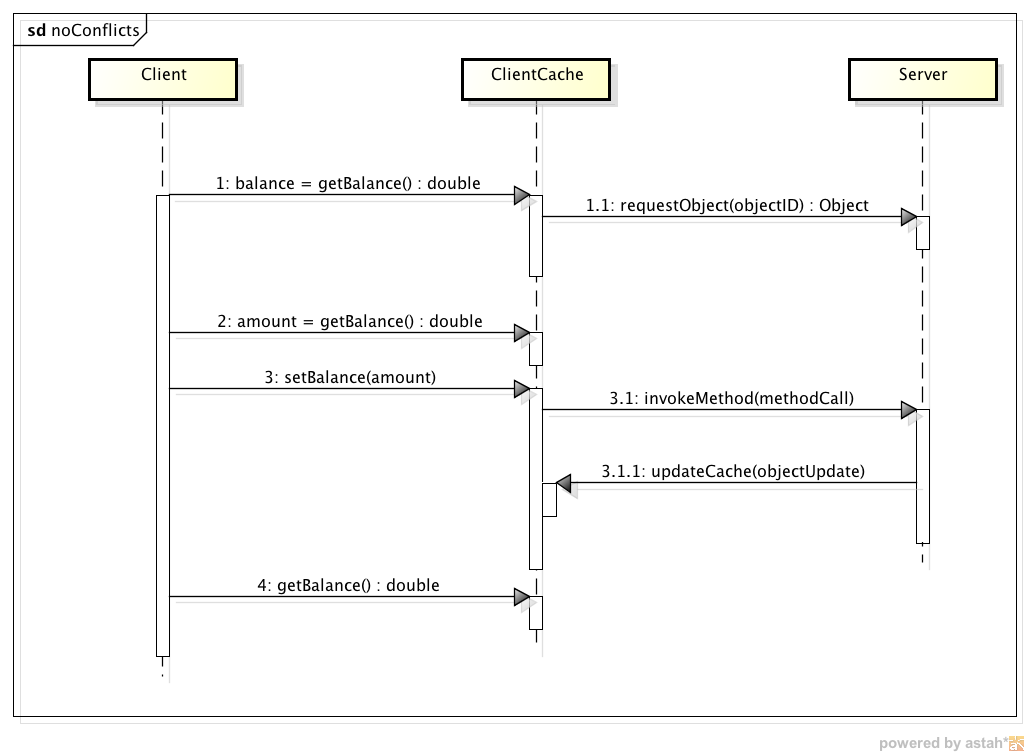
\includegraphics[scale=0.3]{image_testFramework/conflictscenario_noconflict}  
  \caption{Szenario mit einem Client}
  \label{fig:oneclient}
\end{figure}

\subsubsection{Konflikt wird lokal festgestellt}
\label{sec:szenario-mit-zwei}

In diesem Szenario versucht Client 1 ein \texttt{setBalance()} und das Objekt im lokalen Cache von Client 1 wurde seit dem letzen \texttt{getBalance()} im Cache durch ein Update aktualisiert. Der Konflikt kann schon in der Virtual Machine von Client 1 abgefangen werden (siehe \ref{fig:localconflict}).

\begin{enumerate}
\item Client 1 fordert mit \verb|getBalance| ein Objekt an.
\item Client 2 fordert das selbe Objekt auch an.
\item Client 2 ruft \verb|setBalance| auf und verändert das Objekt auf dem Server. Der Server sendet Client 1 ein Update.
\item Client 1 ruft ebenfalls \verb|setBalance| auf. Da sich das Objekt in zwischenzeit geändert hat und Client 1 kein \verb|getBalance()|ausgeführt hat, arbeitet der Client mit veralteten Daten. Der Clientcache vergleicht die aktuelle Versionnummer mit der Versionnummer, die das Objekt beim letzen \verb|getBalance()|-Aufruf hatte. Das Objekt hat inzwischen ein Update erfahren und hat somit eine höhere Versionsnummer. Der Cache wirft eine Exception.

\end{enumerate}

\begin{figure}[h]
  \centering
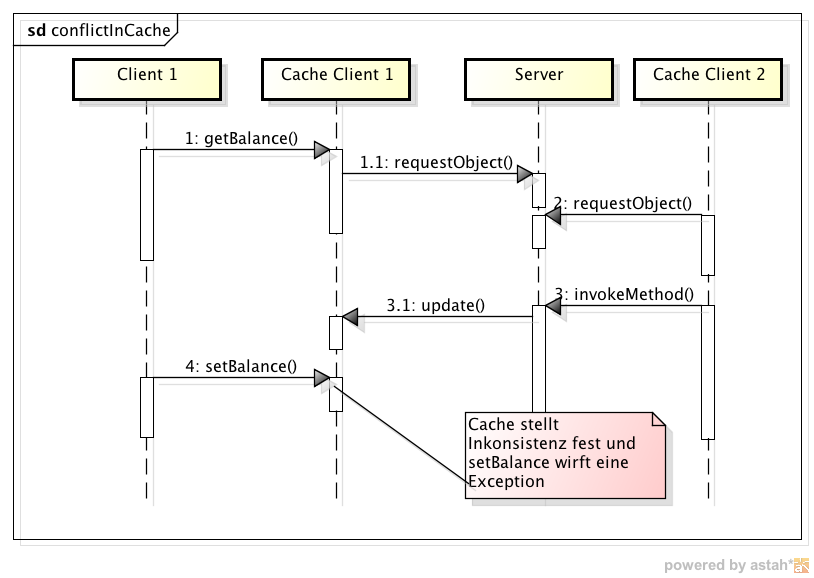
\includegraphics[scale=0.3]{images_objectcaching/conflictInCache}  
  \caption{Konflikt wird in lokal behoben}
  \label{fig:localconflict}
\end{figure}

\subsubsection{Konflikt wird auf Server festgestellt}
\label{sec:konflikt-wird-auf-1}

Eine weitere Möglichkeit in welcher Reihenfolge Methodenaufrufe verarbeitet werden, beinhaltet dass der Server ein \verb|setBalance()|von einem Client erhält bevor er das Update von einem vorangegangenen \texttt{setBalance()} an alle Clients versendet hat. In diesem Fall detektiert der Server die Inkonsistenz. Beide Client haben sich die selbe Version des selben Objektes geholt. Diese Methodaufrufe werden im Sequenzdiagramm \ref{fig:conflictonserver} nicht mehr aufgeführt.

\begin{enumerate}
\item Client 2 sendet ein \verb|setBalance()| an den Server. Bei der Verabeitung dieses Methodenaufrufs macht der Server drei Dinge in dieser Reihenfolge.
  \begin{enumerate}
  \item Methode auf Object ausführen
  \item Update an alle Clients senden
  \item Versionnummern der ConcurrencyControl für jeden Client updat\-en
\end{enumerate}
In diesem Szenario wird der \texttt{setBalance()}-Aufruf unterbrochen bevor er die Versionsnummern updated.
\item Client 1 sendet ebenfalls ein \verb|getBalance()|. Der Cache in Client 1 hat für den Methodenaufruf von Client 2 noch kein Update erhalten. Er wird an den Server weitergeleitet. Der Methodenaufruf trifft beim Server vor dem Versionsnummernupdate des Methodenaufrufs von Client 2 ein. Der Server stellt fest, dass Client 1 noch mit einer alten Version arbeitet und returniert Client 1 eine Exception.
\end{enumerate}

\begin{figure}[h]
  \centering
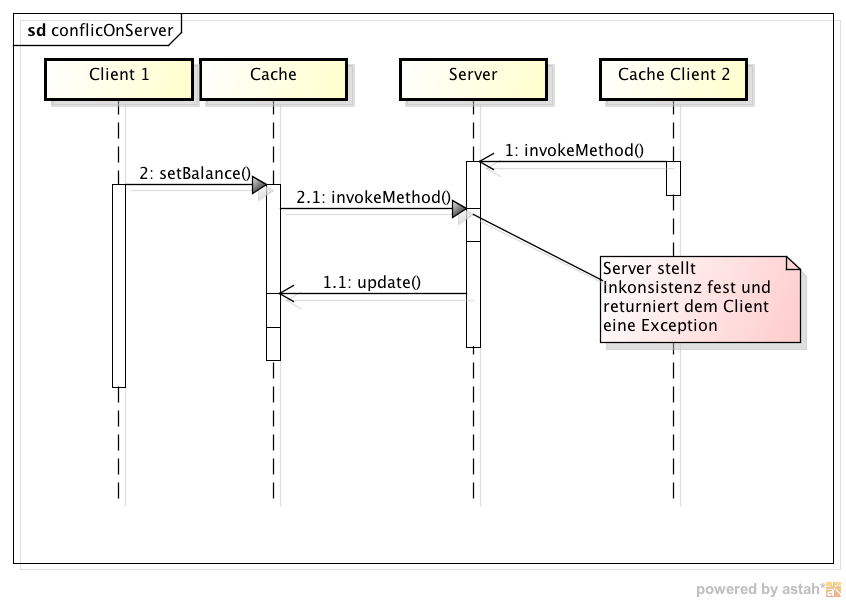
\includegraphics[scale=0.3]{images_objectcaching/conflictOnServer}  
  \caption{Konflikt wird auf Server festgestellt}
  \label{fig:conflictonserver}
\end{figure}

\subsubsection{Update und setBalance überkreuzen sich}
\label{sec:update-und-set}

Bei allen Fällen kann Inkonsistenz festgestellt werden, indem sich der Server und der Clientcache merkt, welche Version an den Client vor dem \verb|setBalance()| heraus\-gegeben wurde und überprüft, ob die Version des Objektes mittlerweile höher ist. Dabei müssen die Versionnummern im Cache und auf dem Server nicht synchron sein. Es gibt jedoch eine Aufrufabfolgemöglichkeit bei der Inkonsistenz entstehen kann (siehe \ref{fig:messagecross}.

\begin{enumerate}
\item Client 2 sendet ein \verb|setBalance()|. Der Server versendet das Update und aktualisiert die Versionsnummern der Clients.
\item Client 1 sendet ebenfalls ein \verb|setBalance()|. Er sendet den Methodenaufruf dem Server bevor er den Update erhalten hat. Zum Zeitpunkt der Ankunft des Methodenaufrufs beim Server, hat der Server aber bereits das Update versendet und die Versionsnummer aktualisiert. Der Methodenaufruf und der Update haben sich also gekreuzt. Da der Server meint, dass Client 1 mit der aktuellen Version arbeitet, wird er den \verb|setBalance()| Aufruf auf dem Objekt ausführen. Es kommt zu einem Lost Update.
\end{enumerate}

\begin{figure}[h]
  \centering
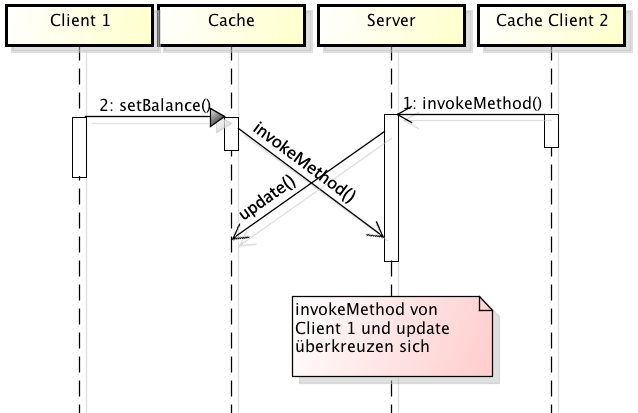
\includegraphics[scale=0.3]{images_objectcaching/conflictCross}  
  \caption{Update und setBalance überkreuzen sich}
  \label{fig:messagecross}
\end{figure}


Um Inkonsistenz bei diesem Szenario zu erkennen und zu verhindern, muss die Nachricht die den \verb|setBalance()| Methodenaufruf enthält, die Versionnummer des Clients, der die Methode aufruft, mitsenden. Ist diese Versionnummer tiefer, als die aktuelle Versionnummer des Objektes wird eine Exception geworfen. Damit die Versionnummern auf Server und auf Client immer synchron sind muss bei einem ObjectRequest die aktuelle Versionnummer an den Client gesendet werden. Bei einem Update wird die Nummer einfach inkrementiert.

Alternative zu der Lösung mit der Versionsnummer, die bei einem Methodenaufruf mitgesendet wird, könnte der Server auch eine Bestätigung des Client, dass er das Update erhalten hat, abwarten und erst nach dieser Bestätigung die Version des entsprechende Client aktualisieren.

